 \documentclass[h]{article}
\usepackage[margin=0.5in]{geometry}
\usepackage{amsfonts} 
\usepackage{textcomp}
 
\usepackage{graphicx}
\usepackage{caption}
\usepackage{subcaption}
\usepackage{float} 
\usepackage{flafter}
\graphicspath{ {./plots/} }
\usepackage{adjustbox}


\newcommand{\cent}{\textcent \hspace{4pt}}
\title{CS 7641 Machine Learning \\ Assignment 3}
\date{Due Sunday April 1st, 2018 11:59pm}
\author{Philip Bale \\ pbale3}

\begin{document}

\maketitle

\section*{Introduction}  
This assignment explores unsupervised learning and dimensitonality reduction.  
It begins by examining clustering algorithms, specifically k-means and 
expectation maximization.  It then proceeds to cover four dimensionality 
reduction algorithms: principal components analysis, individual components 
analysis, randomized projections, and random forests.  After running these six 
algorithms on the original datasets and observing the results, the results are 
then piped into a neural network learner for further examination.

\subsection*{Datasets}  
The datasets chosen were the same datasets chosen for assignment 1.  The first dataset is the US 
permanent visa dataset.  This dataset is interesting due to its potential to aid in the visa application process 
from a cost and time savings potential. It could also enable confidence in those interested in applying for a 
US permanent visa but doubting their chances of acceptance. 
At the end of the day, the goal is it to try to determine the application result before time, money, 
nd other resources are spent.   As before, 6 features are used. 
\\  \\
The second dataset is a home sale price prediction dataset taken from an ongoing 
Kaggle competiton.  This dataset is interesting for two primary reasons: real-world applicability and participating in a Kaggle challenge.
 First, modeling home prices is both a difficult and lucrative task. 
 If one can succesfully model home sale prices on large sets of data, he/she can make large amounts of money 
 investing in real estate when he/she detects outliers in listed price vs. what it is expected to sell for. 
 This applies to flipping, investing, and remodeling. 
 Second, the dataset is part of an ongoing Kaggle competition that does not have a winning solution yet.
  By taking part of the competition, the dataset presents the opportunity to work towards a winning solution 
  and advance ones algorithms over time. As before, 11 features are used. 

\section*{Part 1: Clustering Algorithms}
\subsection*{Introduction}  
K-means clustering is the first algorithm applied to the datasets and expectation maximization is the second. 
 Both algorithms work by clustering: gathering groups of instances together 
 based upon their features.  The rationale is that similar instances will likely 
 be labeled the same way--such as identical visa applications obtaining the same 
 outcome.

\subsection*{1) k-means clustering}  
\subsubsection*{Overview}
K-means works by clustering n instances into k-clusters of similarity using least-squares Euclidean distance
 between the instances.  In practice, the algorithm converges on 'mean' for each cluster that is representative of the 
 members of that cluster.   A variety of cluster sizes were tested to find the best parameters 
 possible.
 
 \begin{figure}[H]
  \minipage{0.33\textwidth}
      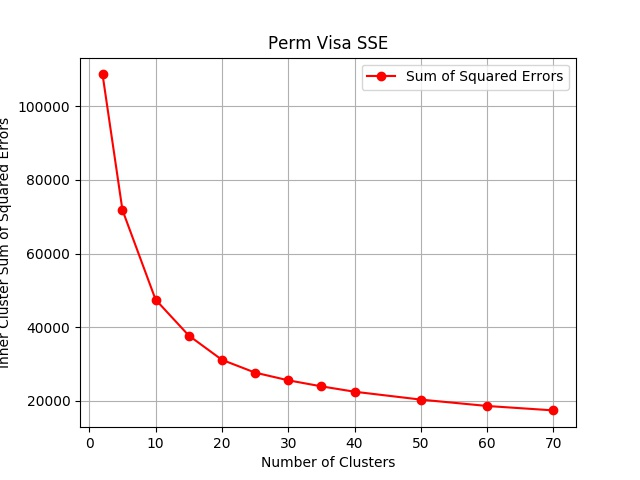
\includegraphics[width=1\textwidth,keepaspectratio]{perm_visa_sse.jpg} 
      \caption*{Perm Visa Sum of Square Errors for Clusters vs. \# Clusters} 
   \endminipage\hfill
      \minipage{0.33\textwidth}
      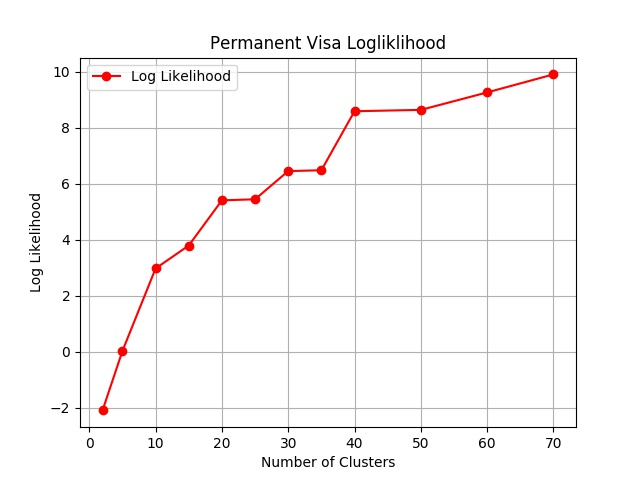
\includegraphics[width=1\textwidth,keepaspectratio]{permanent_visa_logliklihood.jpg} 
      \caption*{Perm Visa Log Liklihood vs. \# Components} 
   \endminipage\hfill
   \minipage{0.33\textwidth}
      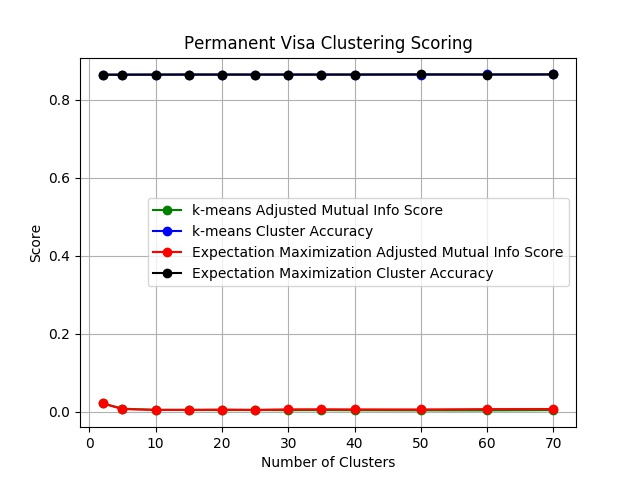
\includegraphics[width=1\textwidth,keepaspectratio]{permanent_visa_clustering_scoring.jpg} 
      \caption*{Perm Visa Scoring for k-means and expectation maximization} 
   \endminipage\hfill
\end{figure}
 \begin{figure}[H]
  \minipage{0.33\textwidth}
      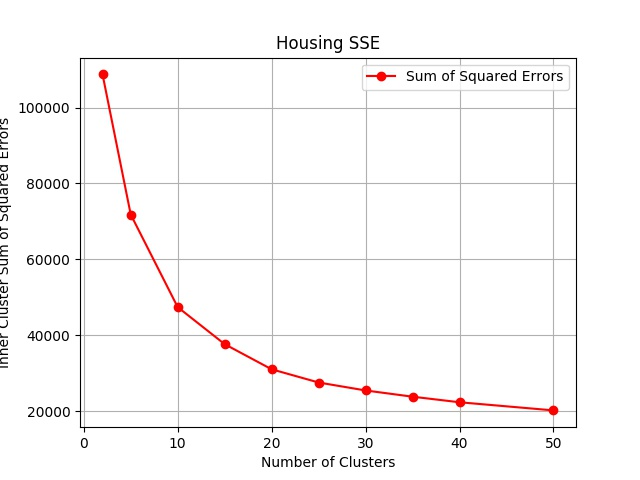
\includegraphics[width=1\textwidth,keepaspectratio]{housing_sse.jpg} 
      \caption*{Housing Sum of Square Errors for Clusters vs. \# Clusters} 
   \endminipage\hfill
   \minipage{0.33\textwidth}
      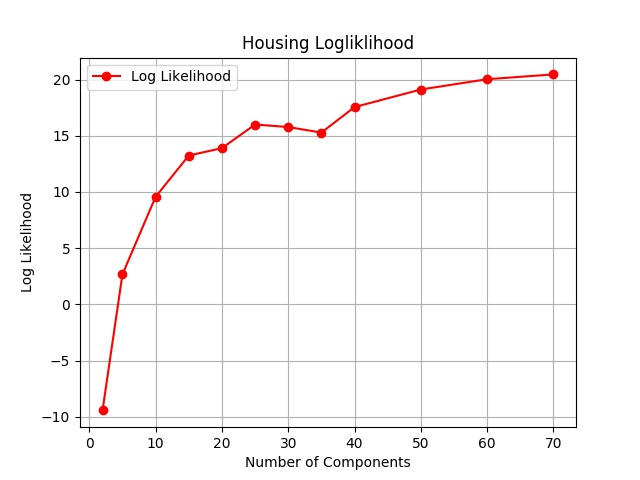
\includegraphics[width=1\textwidth,keepaspectratio]{housing_logliklihood.jpg} 
      \caption*{Housing Log Liklihood vs. \# Components} 
   \endminipage\hfill
   \minipage{0.33\textwidth}
      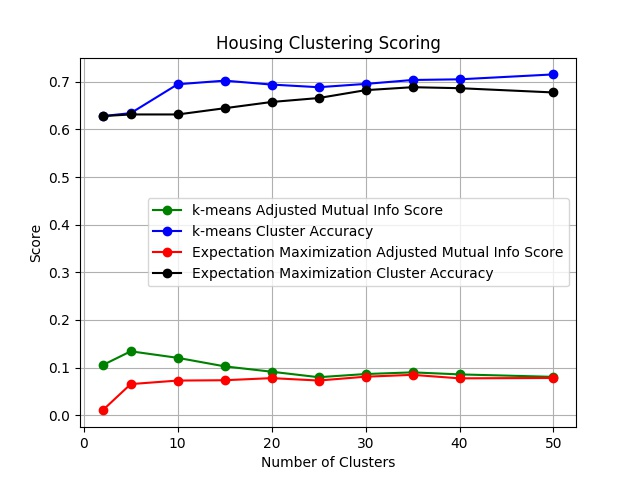
\includegraphics[width=1\textwidth,keepaspectratio]{housing_clustering_scoring.jpg} 
      \caption*{Housing Scoring for k-means and expectation maximization} 
   \endminipage\hfill
\end{figure}

\subsubsection*{k-Means Analysis}
Observing the graphs above, it is clear to see that varying the number of clusters used 
has a clear impact on the performance of k-Means clustering.  For both datasets, as the number of 
clusters increases, the clusters are more able to represent the data. Logically, 
there are instances where increasing number of clusters will decrease the 
accuracy instead of increasing it, such as when just starting out and before 
convergence (using Euclidean distance for converge properties).
\\ \\
The first measurement used to determine the effectiveness is the sum of square 
errors (SSE).  The SSE measures how far away an instance data point is from the mean of its cluster.
As the number of clusters increases, the SSE noticably drops and then converges.  This 
makes sense because at a certain point, adding more clusters is overfitting and 
not necessary to get the all training data into its best possible fit.
\\ \\ 
From the scoring data, it is shown that the permanent visa data, performs remarkably well with a small number of 
clusters and does not show any noticable improvement by increasing clusters.  
This is due to the fact that the permanent visa data is extremely homogenous and 
does not contain many outliers at all.   On the other hand, the housing price 
data is much more susceptible to changes in number of clusters.  As the number 
of clusters increases, the testing data gradually increases in accuracy before leveling off.  
Since the housing data is much more varied and complex, there are intricacies of 
the data that require more clusters to capture well.


\begin{figure}[H] 
\begin{tabular}{ | c | c  | c | c | c | c | c | c| c| c| c| c| c | } 
\hline
\textbf{ # Clusters } & \textbf{2} & \textbf{5} & \textbf{10} & \textbf{15} & \textbf{20} & \textbf{25} & \textbf{30} & \textbf{35} & \textbf{40} & \textbf{50} & \textbf{60} & \textbf{70}   \\
\hline
\textbf{PERM VISA} \\ \hline
\textbf{SSE} &  108717 & 71834 & 47453 & 37701 & 31090 & 27611 & 25517 & 23874 & 22410 & 20267 & 18532 & 17331 \\ \hline
\textbf{Log Liklihood} & -9.44 & 2.67 & 9.57 & 13.25 & 13.90 & 16.01 & 15.78 & 15.29 & 17.56 & 19.12 & 20.04 & 20.47 \\ \hline
\textbf{k-Means AMI} & 0.022 & 0.008 & 0.005 & 0.005 & 0.004 & 0.005 & 0.004 & 0.004 & 0.004 & 0.004 & 0.004 & 0.004 \\ \hline
\textbf{k-Means ACC} & 0.865 & 0.865 & 0.865 & 0.865 & 0.865 & 0.865 & 0.865 & 0.865 & 0.865 & 0.865 & 0.865 & 0.865 \\ \hline
\textbf{EM AMI} & 0.022 & 0.007 & 0.005 & 0.005 & 0.006 & 0.005 & 0.006 & 0.007 & 0.006 & 0.006 & 0.007 & 0.007 \\ \hline
\textbf{EM ACC} & 0.865 & 0.865 & 0.865 & 0.865 & 0.865 & 0.865 & 0.865 & 0.865 & 0.865 & 0.865 & 0.865 & 0.865 \\ \hline
\\
\textbf{HOUSING} \\ \hline
\textbf{SSE} & 14840 & 10217 & 8265 & 7256 & 6589 & 6106 & 5687 & 5339 & 5063 & 4589 & 4276 & 4024 \\ \hline
\textbf{Log Liklihood} & -2.09 & 0.03 & 2.97 & 3.79 & 5.41 & 5.44 & 6.45 & 6.48 & 8.59 & 8.63 & 9.26 & 9.90 \\ \hline
\textbf{k-Means AMI} & 0.105 & 0.134 & 0.120 & 0.103 & 0.091 & 0.080 & 0.086 & 0.090 & 0.086 & 0.081 & 0.083 & 0.081 \\ \hline
\textbf{k-Means ACC} & 0.628 & 0.634 & 0.695 & 0.702 & 0.694 & 0.688 & 0.695 & 0.704 & 0.705 & 0.715 & 0.719 & 0.726 \\ \hline
\textbf{EM AMI} & 0.010 & 0.065 & 0.073 & 0.073 & 0.078 & 0.073 & 0.081 & 0.085 & 0.077 & 0.078 & 0.065 & 0.064 \\ \hline
\textbf{EM ACC} & 0.628 & 0.631 & 0.631 & 0.644 & 0.657 & 0.666 & 0.682 & 0.688 & 0.686 & 0.677 & 0.673 & 0.679 \\ \hline
\end{tabular}
\caption*{Table of Housing Data Results for Cluster } 
\end{figure}

\subsection*{2) Expectation Maximization}  
\subsubsection*{Overview}
Expectation Maximization is the second algorithm applied to the datasets and, 
similar to k-means, is a clustering algorithm.  Expectation Maximization works 
by iteratively finding the maximum liklihood of parameters leading to a labeling 
of an instance despite possibly not having all data or parameters.  For our 
examples, we used Scikit-learn's Gaussian mixture models to implement the 
Expectation Maximization algorithm.  A varying number of mixture components (or number of distributions) were 
used to determine the best possible parameters for the clustering.

\subsubsection*{Expectation Maximization Analysis}
Expectation maximization performed only slightly worse than k-means on the 
datasets.  Insterad of using a sum of square errors calculation, a log liklihood 
is calculated to effectively determine the probability of succesful labeling.  
Interestingly, the housing dataset converges quite quickly to a near-peak log 
liklihood where as the permanent visa dataset takes a bit longer.  This makes 
sense, as the permanent visa dataset is much larger and while an indicitor of 
classification performance and determining factor for component count, it does not gaurantee how well the 
algorithm will perform using such settings.
\\ \\
In terms of scoring, while k-means performed slightly better, it isn't by 
much for the housing dataset--and it was insignificantly better for the 
permanent visa dataset.  The adjusted mutual info score, which helps to 
determine the differences between clusters while accounting for chance, also 
performs similarly for expectation maximization compared to k-means.  Overall, 
while k-means performed better in our trials, it is reasonable to believe 
datasets exist that would fare better using expectation maximization.







 
\section*{Part 2: Dimensionality Reduction Algorithms}
\subsection*{ Introduction}  
Part 2 deals with dimensionality reduction algorithms.  The four algorithms used 
are principal components analysis, individual components analysis, randomized projections, and random 
forests.  After running the algorithms on both datasets, an analysis is provided 
on the results.  Later, we will take the results of the dimensionality reduction 
algorithms and use them as inputs to a neural network.

\subsection*{1) Principal Components Analysis (PCA)}  
\subsubsection*{Overview}
The first dimenstionality reductation algorithm, Principal component analysis is a statistics approach to finding vectors that 
maximize variance and thus help to determine components that are correlated.  Each subsequent component is found with the intent to be 
orthoganal to the preceding component.  The resulting eigenvalue matrix from PCA 
is therefore maximized for covariance.

 \begin{figure}[H]
  \minipage{0.49\textwidth}
      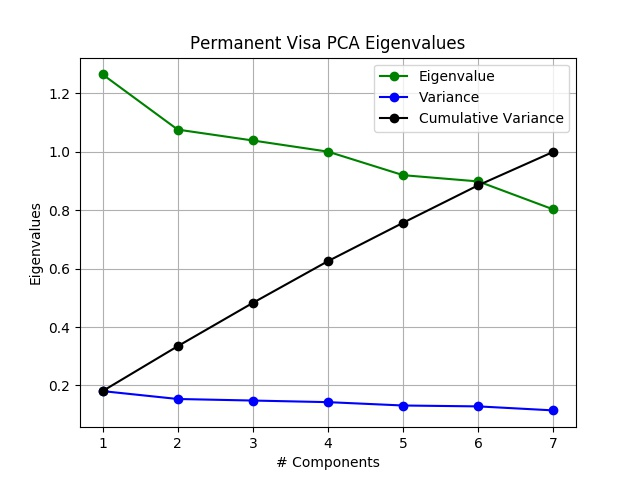
\includegraphics[width=1\textwidth,keepaspectratio]{permanent_visa_pca_eigenvalues.jpg} 
      \caption*{Permanent Visa Principal Components Analysis } 
   \endminipage\hfill
    \minipage{0.49\textwidth}
      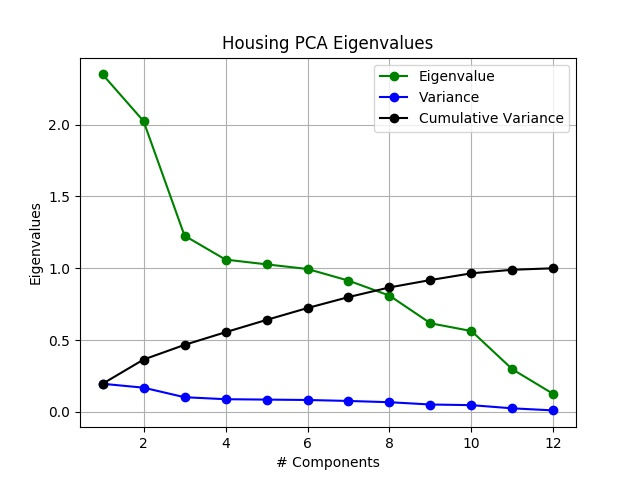
\includegraphics[width=1\textwidth,keepaspectratio]{housing_pca_eigenvalues.jpg} 
      \caption*{Housing Principal Components Analysis } 
   \endminipage\hfill
\end{figure}

\subsubsection*{Analysis}
Principal component analysis seeks to reduce the number of dimensions in the data without sacrificing data quality.  The prinicipal component analysis results show that both the eigenvalues and the variance decrease for 
both datasets as the number of components is increases.  For the permanent visa 
dataset, the size of the eigenvalues is consistant with a slight continous decrease.  In the case that there was a sharp decrease and then level off,
it would indicate that there are features that are potentially unnecessary and removable.  Since the level off is gradual, 
it indicates that each feature is important to representing the initial data.  While the housing 
dataset has a sharp very initial drop, it then has a continous downwards trend for its eigenvalues, 
also indicating that removing too many features may not be a wise thing to do.
\\ \\
The variance graphs also provide interesting views into the ability of PCA to reduce 
dimensionality without sacrificing data quality.  While the housing dataset 
indiciates a higher variance between different features, the permanent visa 
dataset proves to be more evenly distributed.  Since we are trying to maximize 
variance between the different components (so that we most accurately represent the higher dimension 
data), we want to choose a number of components that demonstrates such.  For 
the permanent visa dataset, that number appears to be around 5 components and for 
the housing dataset it apepars to be around 9 components.

\subsection*{2) Independent Components Analysis (ICA)}  
\subsubsection*{Overview}
The second dimensionality reduction algorithm, independent components analysis, 
is an approach to separating a mixture of a data into appropriate subcomponents. 
 As discussed in lecture, a good example of what ICA is used for is the cocktail problem; where one needs to 
 separate various sounds into their sources: a tv show, humans, car noises, etc.  
  Kurtosis is used as a measurement of how gaussian the derived components 
  are.
  

 \begin{figure}[H]
  \minipage{0.49\textwidth}
      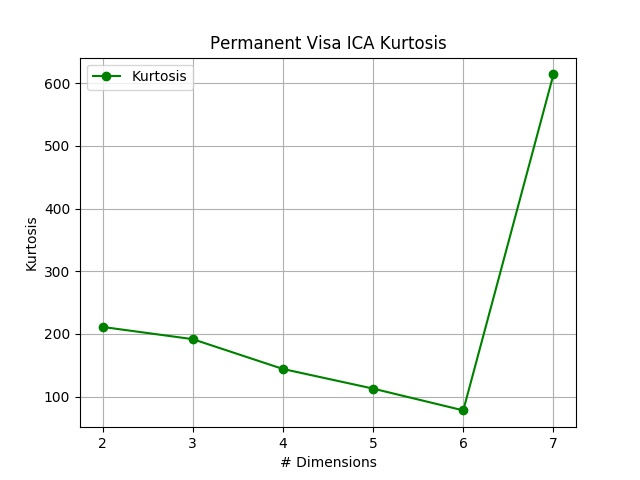
\includegraphics[width=1\textwidth,keepaspectratio]{permanent_visa_ica_kurtosis.jpg} 
      \caption*{Permanent Visa Independent Components Analysis } 
   \endminipage\hfill
    \minipage{0.49\textwidth}
      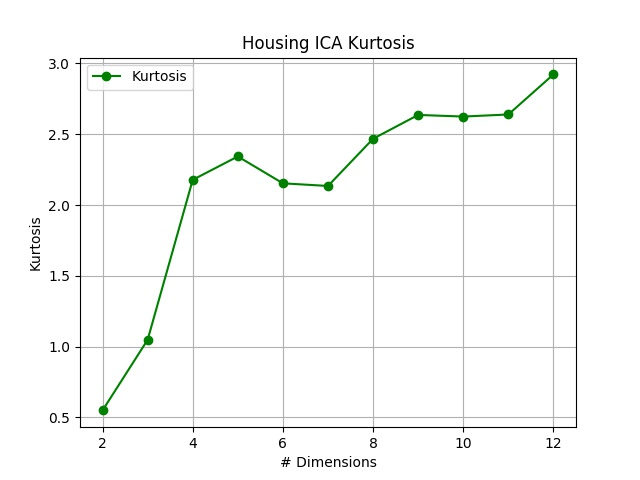
\includegraphics[width=1\textwidth,keepaspectratio]{housing_ica_kurtosis.jpg} 
      \caption*{Housing Independent Components Analysis } 
   \endminipage\hfill
\end{figure}


\subsubsection*{Analysis}
While PCA sought to maximize variance, ICA seeks to separate mixed data into 
subcomponents.  As a dimensionality aglorithm, independent components analysis also wants to minimize 
dimesionality while preserving data quality.  Using the kurtosis measurement, 
we are able to measure the spikiness of the data distribution.  It's important to note that kurtosis is 
sensitive to outliers and therefore not always robust to measuring gaussianity. 
\\ \\ 
The parameter to tune was number of components (dimensions).  Similar to PCA, it is observed that the permanent visa dataset is significantly 
more homogenous then the housing dataset.  It also suggest that 5 dimensions 
be kept for the permanent visa dataset and approximately 5-9 for the housing 
dataset.


\subsection*{3) Randomized Projections}  
\subsubsection*{Overview}
The third dimensionality reduction algorithm, randomized projections, is an 
approach that randomly generates a projection matrix that attempts to create a 
lower dimension representation of the data that is approximately accurate to 
its original state.  By varying the number of components to project, we can run 
varoius tests on how well the lower dimension data captures the original.

 \begin{figure}[H]
  \minipage{0.49\textwidth}
      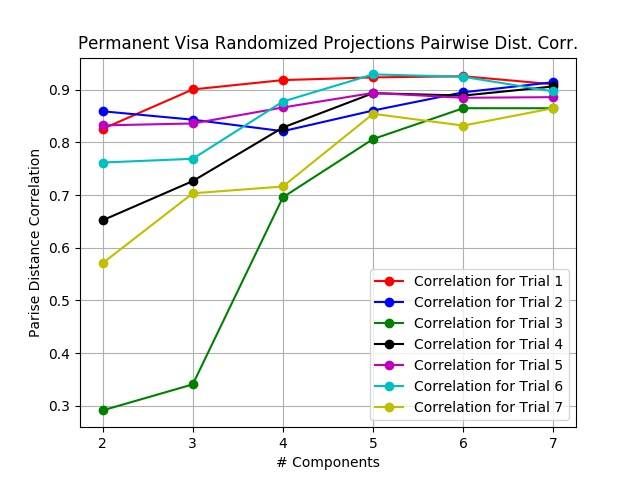
\includegraphics[width=1\textwidth,keepaspectratio]{permanent_visa_randomized_projections_pairwise_distpt_corrpt.jpg} 
      \caption*{Permanent Visa Randomized Projections Pairwise Correlation } 
   \endminipage\hfill
    \minipage{0.49\textwidth}
      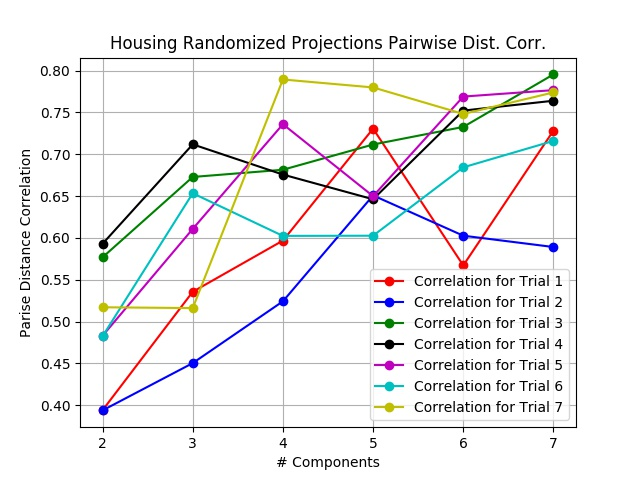
\includegraphics[width=1\textwidth,keepaspectratio]{housing_randomized_projections_pairwise_distpt_corrpt.jpg} 
      \caption*{Housing Randomized Projections Pairwise Correlation} 
   \endminipage\hfill
\end{figure}
 \begin{figure}[H]
  \minipage{0.49\textwidth}
      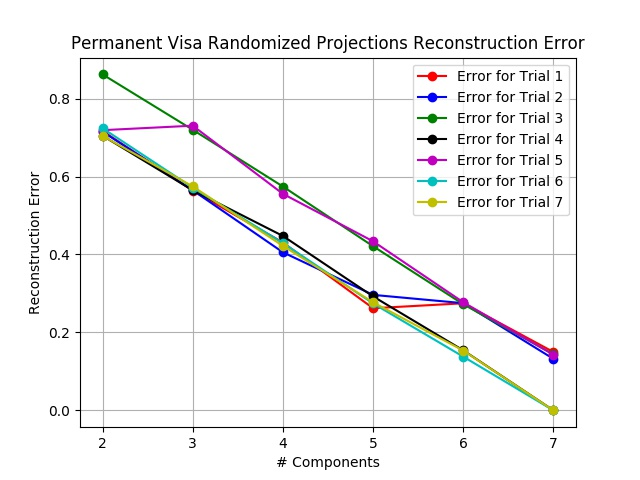
\includegraphics[width=1\textwidth,keepaspectratio]{permanent_visa_randomized_projections_reconstruction_error.jpg} 
      \caption*{Permanent Visa Randomized Projections Reconstruction Error } 
   \endminipage\hfill
    \minipage{0.49\textwidth}
      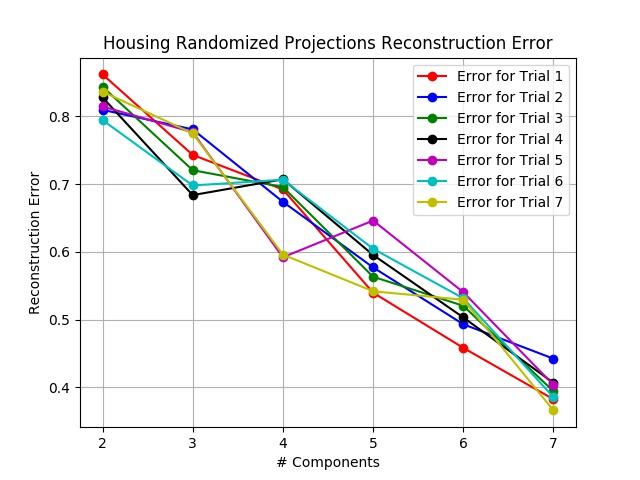
\includegraphics[width=1\textwidth,keepaspectratio]{housing_randomized_projections_reconstruction_error.jpg} 
      \caption*{Housing Randomized Projections Reconstruction Error} 
   \endminipage\hfill
\end{figure}

\subsubsection*{Analysis}
Randomized projections, of all the dimesionality reduction algorithms, was the 
most susceptible to variation in performance due to its random nature.  In such, 
various trials were run, each varying the random state and maintaining that same random state for a variety of 
number of components.  We ran 10 trials for each dataset (and kept the most relevant 7).  
\\ \\
The first measure used to determine the appropriate 
number of dimensions to reduce to was pairwise distance between the original and 
reduced data.  From the graphs, it is easy to see that the distance (akin to difference in the instances) 
converges around 5 components for the permanent visa dataset and 9-10 for the 
housing dataset.
\\ \\
The second, measurement used was reconstruction error.  For both datasets, the 
reconstuction error decreases signficiantly as the number of dimensions is 
increased.  This makes sense as the more dimensions available, the more easily 
the initial data can be reconstructed.  While reconstruction error doesn't give 
us a clear indicator as to how well a learner will perform on the deconstructed 
data, it does give insight into how much data is thrown away at each reduction 
of dimension.

\subsection*{4) Random Forest Feature Selection}  
\subsubsection*{Overview}
The fourth, and last, dimensionality reduction algorithm, random forest feature selection, is an 
approach that uses an ensemble of decision trees conditioned on different 
features.  By training the decision tree and observing the impact of each 
feature by its ability to classify data correctly, we can select the most 
important features and disregard unimporant features.

 \begin{figure}[H]
  \minipage{0.49\textwidth}
      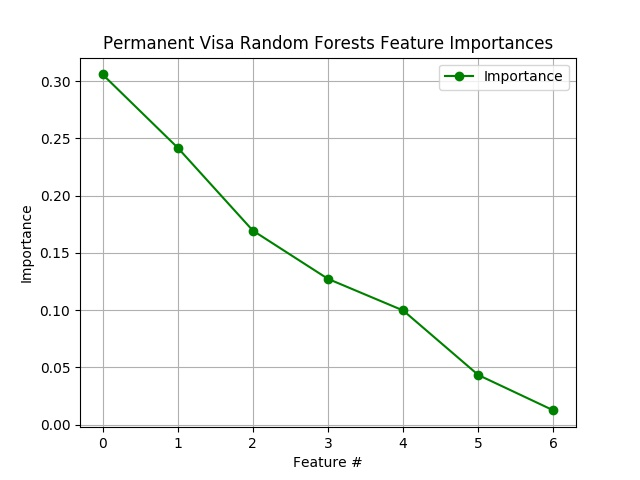
\includegraphics[width=1\textwidth,keepaspectratio]{permanent_visa_random_forests_feature_importances.jpg} 
      \caption*{Permanent Visa Random Forest Feature Importances (Descending Order) } 
   \endminipage\hfill
    \minipage{0.49\textwidth}
      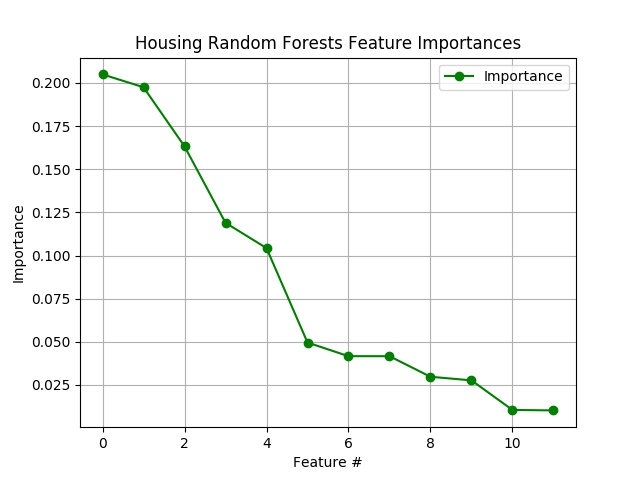
\includegraphics[width=1\textwidth,keepaspectratio]{housing_random_forests_feature_importances.jpg} 
      \caption*{Housing Random Forest Feature Importances (Descending Order)} 
   \endminipage\hfill
\end{figure}

\subsubsection*{Analysis}
The last dimensionality reduction algorithm produces results consistent with the 
others. The number of estimators used was 100 to give a robust learner and all 
class weights were treated equally.  To keep trials consistent, the same random 
state, number of estimators, and initial class weights were used for each 
trial of the random forest feature selector.
\\ \\
For the permanent visa dataset, approximately 5 of the features have high importance 
in terms of a random forest classying data correctly, whereas approximately 9 of 
the features have high importance for the housing dataset.  Interestingly 
enough, the feature importance graph for the housing dataset indicates that there is a quick dropoff 
between 5 features in terms of importance.  These findings are consistent 
with the results of the other dimensionality reduction algorithms.  
\\ \\ 
By using the various algorithms in tandem, it gives us confidence to safely pick 
a dimensionality of 5 for the permanent visa dataset and 9 for the housing 
dataset.


\section*{Part 3: Dimensionality Reduction and Clustering}
\subsection*{Overview}
In this section, clustering algorithms are run on the results of the 
dimensionality reduction algorithms and then compared.  All dimenstionality 
reduction and all clustering algorithms from above are used.

\subsection*{k-Means after Dimensionality Reduction}

 \begin{figure}[H]
  \minipage{.25\textwidth}
      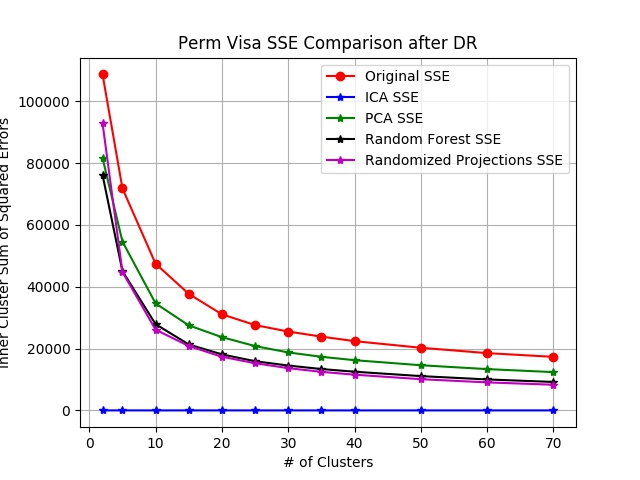
\includegraphics[width=1\textwidth,keepaspectratio]{perm_visa_sse_comparison_after_dr.jpg} 
      \caption*{Perm Visa SSE} 
   \endminipage\hfill
   \minipage{.25\textwidth}
      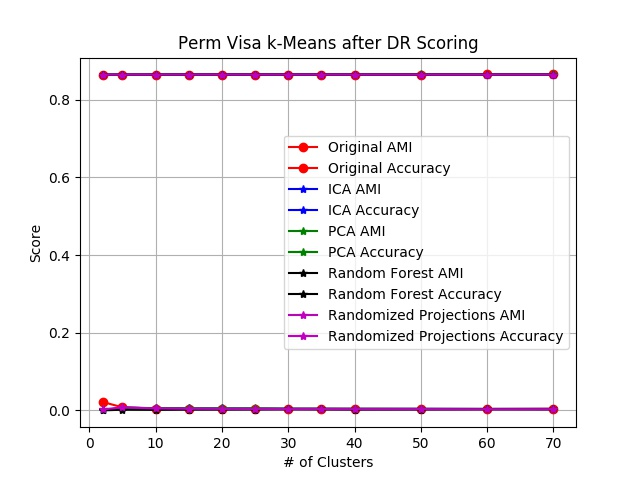
\includegraphics[width=1\textwidth,keepaspectratio]{perm_visa_k-means_after_dr_scoring.jpg} 
      \caption*{Perm Visa Scoring} 
   \endminipage\hfill
  \minipage{.25\textwidth}
      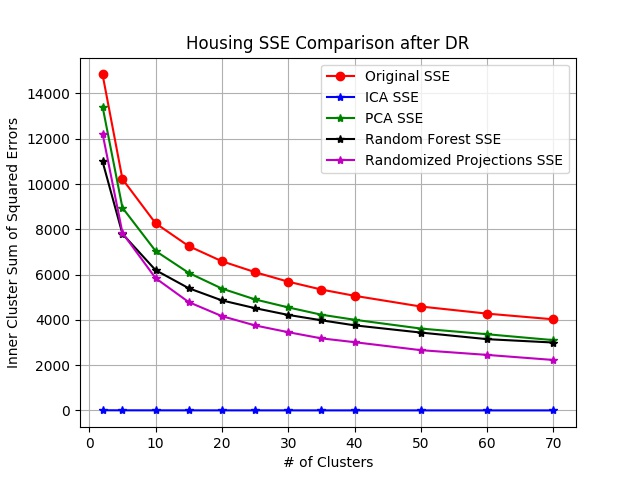
\includegraphics[width=1\textwidth,keepaspectratio]{housing_sse_comparison_after_dr.jpg} 
      \caption*{Housing SSE} 
   \endminipage\hfill
   \minipage{.25\textwidth}
      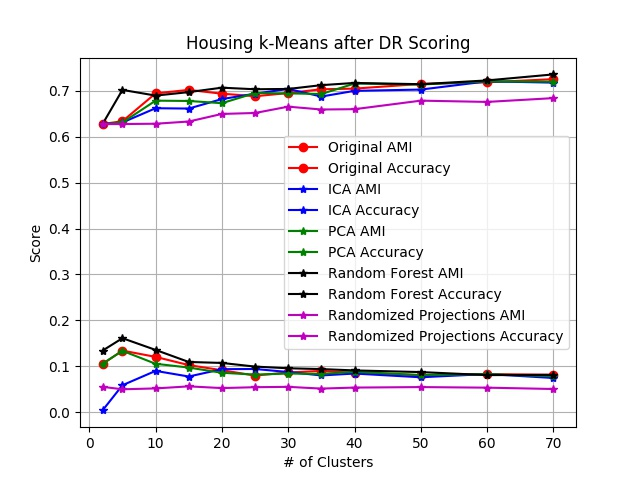
\includegraphics[width=1\textwidth,keepaspectratio]{housing_k-means_after_dr_scoring.jpg} 
      \caption*{Housing Scoring} 
   \endminipage\hfill
  \end{figure}
  
\subsubsection*{Analysis}
Text

\subsection*{Expectation Maximization after Dimensionality Reduction}

 \begin{figure}[H]
  \minipage{.25\textwidth}
      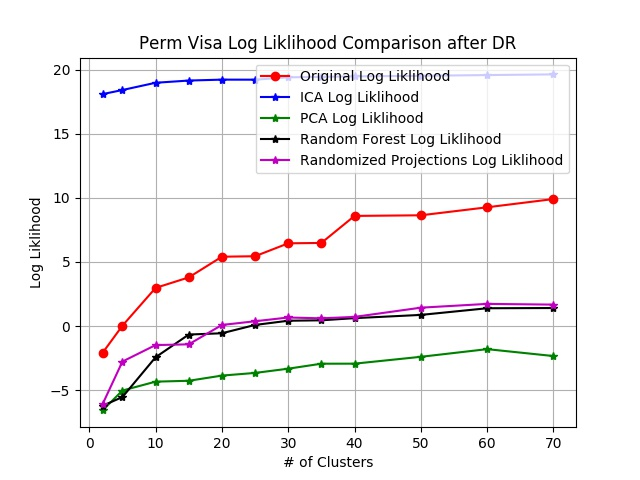
\includegraphics[width=1\textwidth,keepaspectratio]{perm_visa_log_liklihood_comparison_after_dr.jpg} 
      \caption*{Perm Visa Log Liklihood} 
   \endminipage\hfill
   \minipage{.25\textwidth}
      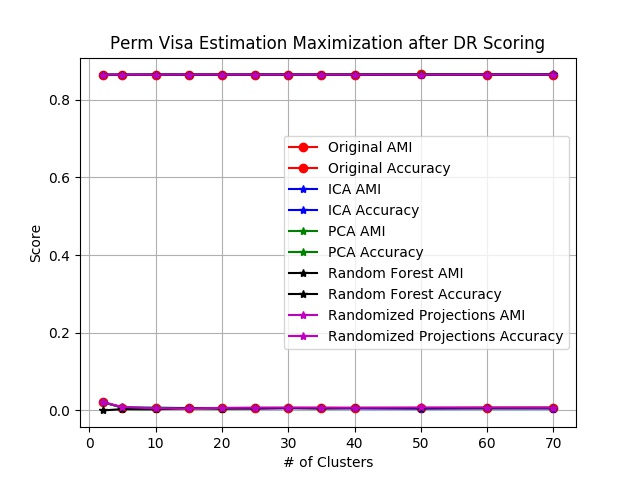
\includegraphics[width=1\textwidth,keepaspectratio]{perm_visa_estimation_maximization_after_dr_scoring.jpg} 
      \caption*{Perm Visa Scoring} 
   \endminipage\hfill
  \minipage{.25\textwidth}
      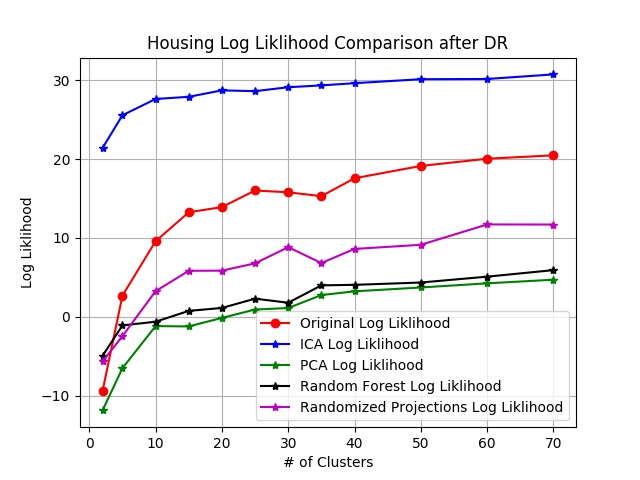
\includegraphics[width=1\textwidth,keepaspectratio]{housing_log_liklihood_comparison_after_dr.jpg} 
      \caption*{Housing Log Liklihood} 
   \endminipage\hfill
   \minipage{.25\textwidth}
      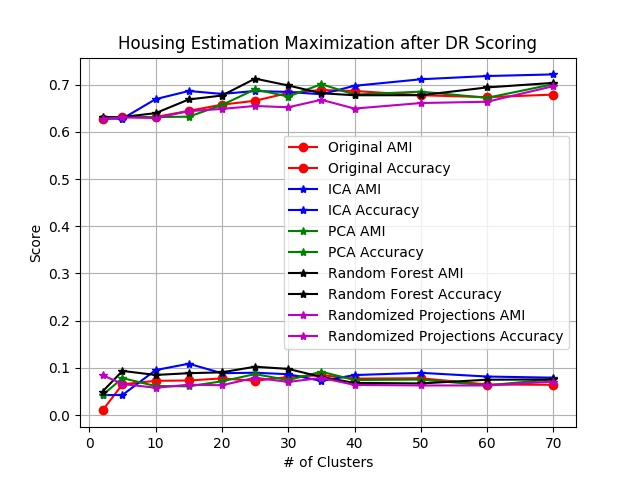
\includegraphics[width=1\textwidth,keepaspectratio]{housing_estimation_maximization_after_dr_scoring.jpg} 
      \caption*{Housing Scoring} 
   \endminipage\hfill
  \end{figure}

\subsubsection*{Analysis}
Text

\section*{Part 4/5: Dimensionality Reduction, Clustering, and Neural Networks}
\subsection*{Overview}
In this section, similar to part 3, neural networks are run on the results of the 
dimensionality reduction algorithms and the clustering algorithms, and then compared.

 \begin{figure}[H]
  \minipage{0.49\textwidth}
      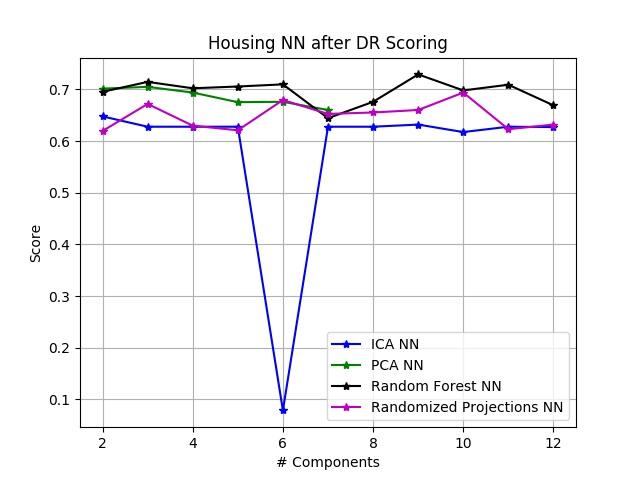
\includegraphics[width=1\textwidth,keepaspectratio]{housing_nn_after_dr_scoring.jpg} 
      \caption*{Housing NN after dimenstionality reduction } 
   \endminipage\hfill
    \minipage{0.49\textwidth}
      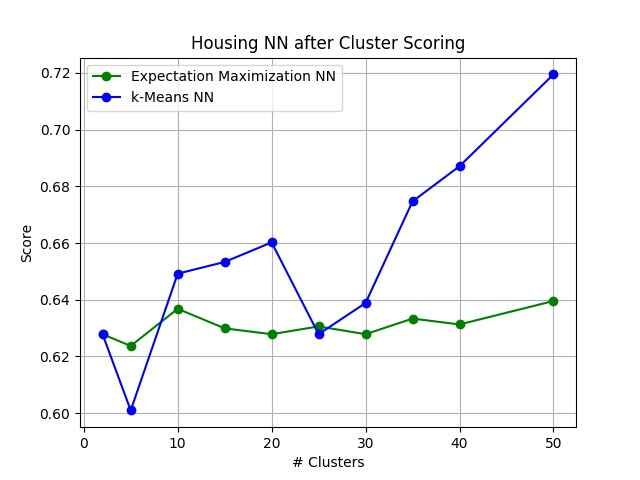
\includegraphics[width=1\textwidth,keepaspectratio]{housing_nn_after_cluster_scoring.jpg} 
      \caption*{Housing NN after clustering} 
   \endminipage\hfill
\end{figure}

\subsubsection*{Dimensionality Reduction + NN Analysis}

\subsubsection*{Clustering + NN Analysis}

\section*{Conclusion}  
Todo conclusion

\end{document}